\documentclass[11pt]{newrucsthesis}

% preamble stuff here
\usepackage{graphicx}                                           % need this for figures etc.
\usepackage{url}                                                % to handle urls 
%\usepackage{natbib}
\usepackage{authordate1-4}                                      % for authordate ref style only
\usepackage{float}												% customised float support
\usepackage{fancyhdr}											% improved header and footer support
\usepackage{makeidx}											% automatic index generation
\usepackage{url}												% URL typesetting
\usepackage{texnames}											% BIBTeX, SliTeX, AMSTeX, PiCTeX and TeXsis logos
\usepackage{verbatim}											% multi-line comments
\usepackage{ifpdf}												% selective setup for PDF compilation
\usepackage{comment}                                            % allows for multi line comments
\usepackage{todonotes}                                          % Adds the todo package, very useful for revision
\usepackage[toc]{glossaries}                                    % Glossary
%\usepackage[style=superborder,toc]{glossaries}                 % Adds a border around glossary



% Math packages
\usepackage{amssymb}											% American Mathematical Society symbols
\usepackage{amsmath}											% American Mathematical Society environments
\usepackage{algorithm}
\usepackage[noend]{algpseudocode} 

%%%%%%%%%%%%%%%%%%%%%%%%%%%%%%%%%%%%%%%%%%%%%%%%
%%%%%%%%%%%% Glossary section %%%%%%%%%%%%%%%%%%
%%%%%%%%%%%%%%%%%%%%%%%%%%%%%%%%%%%%%%%%%%%%%%%%
\setacronymstyle{long-short}

%%%%%%%%%%%%%%%%%%%%%%%%%%%%%%%%%%%%%%%%%%%%%%%%%%%
%% Add all glossary entries here
%% Usage in thesis: \gls{adb}
%%%%%%%%%%%%%%%%%%%%%%%%%%%%%%%%%%%%%%%%%%%%%%%%%%%

\newacronym{adb}{ADB}{Adroid Debugging Bridge}
\newacronym{sdr}{SDR}{Software Defined Radio}

\makenoidxglossaries

%%%%%%%%%%%%%%%%%%%%%%%%%%%%%%%%%%%%%%%%%%%%%%%%
%%%%%%%%%%% Create references %%%%%%%%%%%%%%%%%%
%%%%%%%%%%%%%%%%%%%%%%%%%%%%%%%%%%%%%%%%%%%%%%%%
\renewcommand\bibname{References}


%%%%%%%%%%%%%%%%%%%%%%%%%%%%%%%%%%%%%%%%%%%%%%%%
%%%%%%%%%%%% PDF settings in pdfsettings.tex %%%
%%%%%%%%%%%%%%%%%%%%%%%%%%%%%%%%%%%%%%%%%%%%%%%%
%%%%%%%%%%%%%%%%%%%%%%%%%%%%%%%%%%%%%%%%%%%%%%%
%%%%    PDF Settings   %%%%%%%%%%%%%%%%%%%%%%%%
%%%%%%%%%%%%%%%%%%%%%%%%%%%%%%%%%%%%%%%%%%%%%%%
\ifpdf

% PDFLaTeX-specific packages

\usepackage[
	pdftex,															% hyperlinked references for PDF output
	bookmarks=true,												% (option) build bookmarks
	bookmarksnumbered=true										% (option) add section numbers to bookmarks
]{hyperref}

\usepackage{pdfpages}											% required for PDF watermarking
\usepackage{epstopdf}											% automatic conversion of EPS images
\usepackage[pdftex]{thumbpdf}									% thumbnail generation for PDF files
\usepackage{pdflscape}											% required by thumbpdf
\usepackage[all]{hypcap}										% correct PDF figure links to top of image

\usepackage[printonlyused]{acronym}


% setup options for hyperlinks

\hypersetup{
	pdfhighlight=/N,											% (option) no visual cue on clicking link
	pdffitwindow=true,											% (option)
	pdfstartview=Fit,											% (option) fit initial view to page
	plainpages=false,											% (option) prevent hyperref page number changes
	breaklinks=true,											% (option) allow link breaking across lines
	colorlinks=true,											% (option) color link text only (no borders)
	pageanchor=false,											% (option) turns off page referencing for title page
	linkcolor=black,												% (option) internal link color
	citecolor=black,												% (option) citation link color
	filecolor=black,												% (option) file link color
	menucolor=black,												% (option) Acrobat menu link color
	%pagecolor=black,												% (option) page link color
	urlcolor=black,												% (option) URL link color
}

% PDF meta-data settings
%%%%%%%%%%%%%%%%%%%%%%%%%%%%%%%%%%%%%%%%%%%%%%%%%
%%%        Fill in personal meta-data         %%%
%%%%%%%%%%%%%%%%%%%%%%%%%%%%%%%%%%%%%%%%%%%%%%%%%
\hypersetup{
	pdftitle    = {},
	pdfauthor   = {},
	pdfsubject  = {},
	pdfkeywords = {},
}

% force LaTeX-compliant spacing

\pdfadjustspacing=1

%%%%%%%%%%%%%%%%%%%%%%%%%%%%%%%%%%%%%%%%%%%%%%%%%
%%%       DVI/PostScript-Specific setup       %%%
%%%%%%%%%%%%%%%%%%%%%%%%%%%%%%%%%%%%%%%%%%%%%%%%%

\else

\usepackage{graphicx}											% EPS graphics

\fi
%%%%%%%%%%%%%%%%%%%%%%%%%%%%%%%%%%%%%%%%%%%%%%%
%%%%    PDF Settings End  %%%%%%%%%%%%%%%%%%%%%
%%%%%%%%%%%%%%%%%%%%%%%%%%%%%%%%%%%%%%%%%%%%%%%





\title{Rhodes MSc Thesis Template}
\author{Bob D. Builder}
\date{January 2017}

\begin{document}


%%%%%%%%%%%%%%%%%%%%%%%%%%%%%%%%%%%%%%%%%%%%%%%%
%%%%%%%%%%% Generate cover pages  %%%%%%%%%%%%%% 
%%%%%%%%%%%%%%%%%%%%%%%%%%%%%%%%%%%%%%%%%%%%%%%%
\maketitle

\pagenumbering{roman}

%%%%%%%%%%%%%%%%%%%%%%%%%%%%%%%%%%%%%%%%%%%%%%%%%
%%%% Generates Abstract Page %%%%%%%%%%%%%%%%%%%%
%%%%%%%%%%%%%%%%%%%%%%%%%%%%%%%%%%%%%%%%%%%%%%%%%
\begin{center}
	{\large\bf Put flashy title here}
\end{center}
\begin{center}by\end{center}
\begin{center}
	{Bob D. Builder}\\
	\ifpdf
		E-mail: \href{mailto:bob@builder.co.za}{bob@builder.co.za}
	\else
		E-mail: bob@builder.co.za
	\fi
\end{center}
\vspace{1cm}
\begin{center}{\large\bf Abstract}\end{center}

\textbf{Abstract:} Lorem ipsum sagittis posuere maecenas adipiscing suscipit mi lacinia suspendisse, ante auctor class neque senectus proin lacinia rutrum commodo, fusce quam curabitur neque odio viverra lacinia risus molestie aliquam vivamus ligula morbi ultrices vivamus, nec potenti morbi proin sagittis curabitur nostra, donec rutrum habitant proin arcu.

Nisl sociosqu aliquet ut sit sed luctus ligula ullamcorper donec netus euismod feugiat eu, nunc amet ultricies nam dictum litora vivamus donec urna ipsum enim libero vehicula a lectus aliquam pharetra curabitur a, diam varius sit elementum egestas habitasse, curae in curabitur quam bibendum habitant proin ante leo integer vivamus mi convallis gravida, porta odio libero nisi erat quam pellentesque sapien, auctor ipsum ullamcorper mi enim felis fusce mauris ad accumsan pulvinar ac vestibulum scelerisque, habitasse iaculis aenean mollis blandit tristique orci augue, inceptos sem lacus varius quisque sollicitudin.

Id sapien luctus ad donec hendrerit mollis congue dolor sed, nec volutpat lectus pretium volutpat ligula purus nisi, eleifend morbi rhoncus erat conubia litora lacinia posuere odio sagittis aenean sit tortor fringilla, vehicula ornare leo magna integer, lacinia egestas dapibus eleifend.

\noindent\

\noindent{\bf Keywords:} Awesome, Wow, Coffee

\vfill
\noindent
{\bf\parbox{26.8mm}{Supervisor}:} Prof.~B. Irwin \\* % only provide titles of Prof. or Dr. (not Mr.)
{\bf\parbox{28.55mm}{~}} \\*
%{\bf\parbox{26.8mm}{Supervisor}:} Prof.~S. U. P. Visor \\* % if you only have a single supervisor
{\bf\parbox{26.8mm}{Department}:} Department of Computer Science \\*
{\bf\parbox{26.8mm}{Degree}:} Master of Science

%%%%%%%%%%%%%%%%%%%%%%%%%%%%%%%%%%%%%%%%%%%%%%%%%
%%%%%%%%%%%%%%%%%%%%%%%%%%%%%%%%%%%%%%%%%%%%%%%%%

\section*{\ackname}

I would like to thank : 

\begin{itemize}
\item Monty Python
\item Sauron
\item Gandalf
\item Frodo
\item Samwise
\item Darth Vader
\end{itemize}

\begin{acm}
    Thesis classification under the ACM Computing Classification System\footnote{http://www.acm.org/about/class/2012/} (2012 version, valid through 2017):
    
    
\todo[inline]{Figure out how to do this properly. On-line guide available at http://www.acm.org/about/class/2012/ }
    %    \ccsdesc[500]{Security and privacy  Denial-of-service attacks}
    %    \ccsdesc[100]{Security and privacy Mobile and wireless security}
\end{acm}

%\ccsdesc[500]{Security and privacy~Denial-of-service attacks}
%\ccsdesc[100]{Security and privacy~Mobile and wireless security}

%\printccsdesc







%%%%%%%%%%%%%%%%%%%%%%%%%%%%%%%%%%%%%%%%%%%%%%%%
%%%%%%%%%%%% All lists declarations %%%%%%%%%%%%
%%%%%%%%%%%%%%%%%%%%%%%%%%%%%%%%%%%%%%%%%%%%%%%%
%\printnoidxglossaries                       % List of Glossary entries
\tableofcontents                            % List all Chapters and Sections
\listoffigures                              % List all Figures
\addcontentsline{toc}{chapter}{\listfigurename}
\listoftables                               % List of Table
\addcontentsline{toc}{chapter}{\listtablename}
\listofalgorithms                           % List of algorithms
\addcontentsline{toc}{chapter}{\listalgorithmname}
%\listofequations                           % List of equations
\printnoidxglossaries                       % List of Glossary entries

\pagenumbering{arabic}

 % Include all the chapters for thesis
 % It might be useful to disable chapters with long compile times
%%%%%%%%%%%%%%%%%%%%%%%%%%%%%%%%%%%%%%%%%%%%%%%%%
%%%%%%%%%%%%%%%%%%%%%%%%%%%%%%%%%%%%%%%%%%%%%%%%%

\chapter{Introduction}
\label{chap:intro}

%%%%%%%%%%%%%%%%%%%%%%%%%%%%%%%%%%%%%%%%%%%%%%%%%
%%%%%%%%%%%%%%%%%%%%%%%%%%%%%%%%%%%%%%%%%%%%%%%%%
\section{Proposal}
\label{sec:proposal}

\section{Hypothesis}
\label{sec:hype}


\section{Research Questions}
\label{sec:researchQuestions}


\begin{itemize}
    \item Where is my coffee?
    \item Is there enough coffee?
    \item \ldots clearly not.
\end{itemize}

Steps required to make coffee

\begin{enumerate}
    \item Hire an intern.
    \item Request coffee from intern.
\end{enumerate}


Example of multiple citation \citet{schneier2015,doctorow2011}. Example of single citation \cite{doctorow2011}. First occurrence of acronym \gls{adb}. Second occurrence \gls{adb}.

\subsubsection{Max level indentation}
If you need more indentation than this something went very wrong.

If you are ready for some more complex \LaTeX, have a look at Equation \ref{eq:OpinionCalc} or Algorithm \ref{alg:Lorenz} in Chapter \ref{chap:exp}

%%%%%%%%%%%%%%%%%%%%%%%%%%%%%%%%%%%%%%%%%%%%%%%%%
%%%%%%%%%%%%%%%%%%%%%%%%%%%%%%%%%%%%%%%%%%%%%%%%%

\chapter{Literature Review}
\label{chap:lit}

%%%%%%%%%%%%%%%%%%%%%%%%%%%%%%%%%%%%%%%%%%%%%%%%%
%%%%%%%%%%%%%%%%%%%%%%%%%%%%%%%%%%%%%%%%%%%%%%%%%
\section{Coffee}

How do I make coffee again, please view Section \ref{sec:researchQuestions}.
%%%%%%%%%%%%%%%%%%%%%%%%%%%%%%%%%%%%%%%%%%%%%%%%%
%%%%%%%%%%%%%%%%%%%%%%%%%%%%%%%%%%%%%%%%%%%%%%%%%

\chapter{Experimental Setup}

\label{chap:exp}

\section{Random maths}
An example equation: 

\begin{equation}
    \label{eq:OpinionTriangle}
    \begin{aligned}
        b+d+u=1, \{b,d,u\}\in[0,1]
    \end{aligned}
\end{equation}

\begin{equation}
    \label{eq:OpinionGeneral}
    \begin{array}{l l}
    w_p^{A} & =\{b_p^A,d_p^A,u_p^A\} \\
    \text{where,}
    \end{array}
\end{equation}
\begin{equation}
    \label{eq:OpinionCalc}
     w_A^B = \left\{
    \begin{array}{l l}
        b_A^B \dfrac{p}{p+n+u} & \quad \\
        d_A^B \dfrac{n}{p+n+u} & \quad \text{, where } u_A^B \neq  0\\
        u_A^B \dfrac{u}{p+n+u} &
    \end{array} \right.
\end{equation}

An example algorithm: 
\begin{algorithm}
    \label{alg:Lorenz}
	\centering{\fbox{\parbox[]{155mm}{
		\begin{algorithmic}[1]
    	\Require W[ ]- a sorted array of all wealth distributions
    	\Function{LorenzCurve}{W[ ]}
    	
    	   \State $L[ ] $ \Comment{An empty set of equal length to W[ ]}
    	    
    	   \State $currentTotal \gets 0$
            \For {$i\gets 1,W.length()$ }
            
                \State $currentTotal \gets currentTotal + W[i]$
                
                \State $L[i] \gets currentTotal$
            \EndFor
            
            \Return $L[  ]$
        \EndFunction
    \end{algorithmic}
	}}}
	\caption{Pseudo code for calculating Lorenz Curve plot points}
	%\label{alg:Lorenz}
\end{algorithm}


%%%%%%%%%%%%%%%%%%%%%%%%%%%%%%%%%%%%%%%%%%%%%%%%%
%%%%%%%%%%%%%%%%%%%%%%%%%%%%%%%%%%%%%%%%%%%%%%%%%
And here you can see an image of a rarely spotted special snowflake in Figure \ref{fig:snowflake}
\begin{figure}[H]
    \centering
    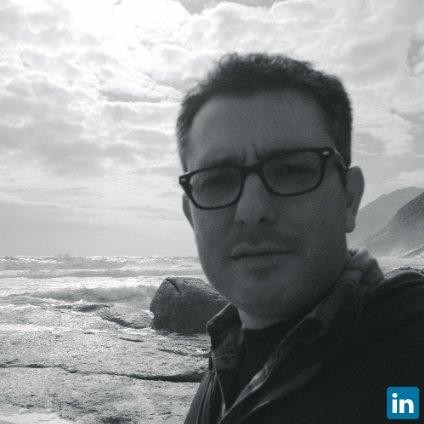
\includegraphics[width=88mm]{chapters/03/images/snow_flake}
    \caption{Special snowflake}
    \label{fig:snowflake}
\end{figure}
%%%%%%%%%%%%%%%%%%%%%%%%%%%%%%%%%%%%%%%%%%%%%%%%%
%%%%%%%%%%%%%%%%%%%%%%%%%%%%%%%%%%%%%%%%%%%%%%%%%

\chapter{Analysis}
\label{chap:analysis}

%%%%%%%%%%%%%%%%%%%%%%%%%%%%%%%%%%%%%%%%%%%%%%%%%
%%%%%%%%%%%%%%%%%%%%%%%%%%%%%%%%%%%%%%%%%%%%%%%%%
%%%%%%%%%%%%%%%%%%%%%%%%%%%%%%%%%%%%%%%%%%%%%%%%%
%%%%%%%%%%%%%%%%%%%%%%%%%%%%%%%%%%%%%%%%%%%%%%%%%

\chapter{Results and Discussion}
\label{chap:result}

%%%%%%%%%%%%%%%%%%%%%%%%%%%%%%%%%%%%%%%%%%%%%%%%%
%%%%%%%%%%%%%%%%%%%%%%%%%%%%%%%%%%%%%%%%%%%%%%%%%
%%%%%%%%%%%%%%%%%%%%%%%%%%%%%%%%%%%%%%%%%%%%%%%%%
%%%%%%%%%%%%%%%%%%%%%%%%%%%%%%%%%%%%%%%%%%%%%%%%%

\chapter{Conclusion}
\label{chap:con}

%%%%%%%%%%%%%%%%%%%%%%%%%%%%%%%%%%%%%%%%%%%%%%%%%
%%%%%%%%%%%%%%%%%%%%%%%%%%%%%%%%%%%%%%%%%%%%%%%%%

\gls{gcd} 

\gls{part} 


%%%%%%%%%%%%%%%%%%%%%%%%%%%%%%%%%%%%%%%%%%%%%%%%
%%%%%%%%%%% Generate Reference list %%%%%%%%%%%%
%%%%%%%%%%%%%%%%%%%%%%%%%%%%%%%%%%%%%%%%%%%%%%%%

%\bibliographystyle{acm}  
%\bibliographystyle{rucsacm}   
\bibliographystyle{ruauthordate}   % also uncomment the usepackage{authordate1-4} above
\label{References}
\bibliography{thesis}   	% load in the info produced from thesis.bib


\end{document}
